%% Artigo COTB 2027 -- Topograf
%% Duas versoes a partir deste arquivo:
%%   topograf_cotb2027.tex       -> versao de avaliacao (anonima)
%%   topograf_cotb2027_final.tex -> versao final (define \versaofinal e inclui este arquivo)
\ifdefined\versaofinal\else\PassOptionsToClass{anonymous}{acmart}\fi
\documentclass[sigconf, nonacm, screen, language=portuguese, language={main=english}]{acmart}

%% \anonfinal{texto na avaliacao}{texto na versao final}
\newcommand{\anonfinal}[2]{\ifdefined\versaofinal#2\else#1\fi}

\AtBeginDocument{%
  \providecommand\BibTeX{{%
    \normalfont B\kern-0.5em{\scshape i\kern-0.25em b}\kern-0.8em\TeX}}}

\usepackage{amsmath}
\usepackage{amsfonts}
\let\Bbbk\relax
\usepackage{amssymb}
\usepackage{booktabs}
\usepackage{multirow}
\usepackage{graphicx}
\usepackage{listings}

\settopmatter{printccs=false, printacmref=false, authorsperrow=2}
\renewcommand\footnotetextcopyrightpermission[1]{}

%% ---------------------------------------------------------------------
%% Cabecalho do evento (mantido do template COTB 2027)
%% ---------------------------------------------------------------------
\makeatletter
\newcounter{cotbNumAuthors}
\let\cotb@originalauthor\author
\renewcommand{\author}[1]{%
  \stepcounter{cotbNumAuthors}%
  \ifnum\value{cotbNumAuthors}=1
    \gdef\cotbFirstAuthorName{#1}%
  \fi
  \cotb@originalauthor{#1}%
}
\makeatother

\newcommand{\cotbEventInfo}{XVIII Computer on the Beach (COTB 2027)\\
  Florianópolis/SC --- 13 a 17 de abril de 2027}

%% Na versao de avaliacao usa \shortauthors ("Anon."): o "et al." do template
%% usaria o nome real do primeiro autor mesmo com a opcao "anonymous".
\newcommand{\cotbHeaderAuthors}{%
  \ifdefined\versaofinal
    \ifnum\value{cotbNumAuthors}>3
      \cotbFirstAuthorName\ et al.%
    \else
      \shortauthors
    \fi
  \else
    \shortauthors
  \fi
}

\setlength{\headheight}{24pt}

\AtBeginDocument{%
  \fancypagestyle{firstpagestyle}{%
    \fancyhf{}%
    \renewcommand{\headrulewidth}{0.4pt}%
    \renewcommand{\footrulewidth}{0pt}%
    \fancyhead[L]{\begin{minipage}[b]{0.62\textwidth}\raggedright
      \scriptsize\cotbEventInfo\end{minipage}}%
    \fancyhead[R]{\begin{minipage}[b]{0.34\textwidth}\raggedleft
      \scriptsize\cotbHeaderAuthors\end{minipage}}%
    \fancyfoot[C]{\if@ACM@printfolios\thepage\fi}%
  }%
  \fancypagestyle{standardpagestyle}{%
    \fancyhf{}%
    \renewcommand{\headrulewidth}{0.4pt}%
    \renewcommand{\footrulewidth}{0pt}%
    \fancyhead[L]{\begin{minipage}[b]{0.62\textwidth}\raggedright
      \scriptsize\cotbEventInfo\end{minipage}}%
    \fancyhead[R]{\begin{minipage}[b]{0.34\textwidth}\raggedleft
      \scriptsize\cotbHeaderAuthors\end{minipage}}%
    \fancyfoot[C]{\if@ACM@printfolios\thepage\fi}%
  }%
  \pagestyle{standardpagestyle}%
}

%% ---------------------------------------------------------------------
%% Listagens da linguagem Topograf
%% ---------------------------------------------------------------------
\lstdefinelanguage{Topograf}{
  morekeywords={terrain,perlin,noise,display,export,as,to,octaves,depth},
  morekeywords=[2]{max,min,above,below,avg,mix},
  sensitive=true,
  morecomment=[l]{//},
  morestring=[b]",
}
\lstset{
  language=Topograf,
  basicstyle=\ttfamily\footnotesize,
  keywordstyle=\bfseries,
  keywordstyle=[2]{},
  commentstyle=\itshape\color{gray},
  columns=fullflexible,
  keepspaces=true,
  frame=tb,
  numbers=left,
  numberstyle=\tiny,
  xleftmargin=1em,
  inputencoding=utf8,
  extendedchars=true,
  literate={á}{{\'a}}1 {é}{{\'e}}1 {í}{{\'i}}1 {ó}{{\'o}}1 {ú}{{\'u}}1
           {ã}{{\~a}}1 {õ}{{\~o}}1 {ç}{{\c{c}}}1 {ê}{{\^e}}1 {ô}{{\^o}}1
           {×}{{$\times$}}1,
}

%% Marcador visivel de pendencia (remover antes da submissao)
\newcommand{\todo}[1]{\textcolor{red}{[\textbf{TODO:} #1]}}

\begin{document}

\title{TopografDSL: A Domain-Specific Language for Composing Perlin Noise into Terrains}
\translatedtitle{portuguese}{TopografDSL: uma linguagem de domínio específico para composição de ruídos Perlin na geração de terrenos}

%% Autores: ocultos no PDF pela opcao "anonymous" do \documentclass.
\author{André Vitor Bastos de Macêdo}
\affiliation{%
  \institution{Instituto Federal Catarinense, Campus Blumenau}
  \city{Blumenau}
  \state{SC}
  \country{Brasil}}
\email{andre.macedo@estudantes.ifc.edu.br}

\author{Gabriel Rodrigues Gonçalves}
\affiliation{%
  \institution{Instituto Federal Catarinense, Campus Blumenau}
  \city{Blumenau}
  \state{SC}
  \country{Brasil}}
\email{gabriel.goncalves@estudantes.ifc.edu.br}

\author{Ricardo de la Rocha Ladeira}
\affiliation{%
  \institution{Instituto Federal Catarinense, Campus Blumenau}
  \city{Blumenau}
  \state{SC}
  \country{Brasil}}
\email{ricardo.ladeira@ifc.edu.br}

\author{Paulo Cesar Rodacki Gomes}
\affiliation{%
  \institution{Instituto Federal Catarinense, Campus Blumenau}
  \city{Blumenau}
  \state{SC}
  \country{Brasil}}
\email{paulo.gomes@ifc.edu.br}

\begin{abstract}
Procedural terrain generation commonly combines layers of Perlin noise,
but these combinations are usually written directly in general-purpose
code, where the intent of each step is buried in loops and errors only
become visible in the generated terrain. This paper presents Topograf, a
textual domain-specific language for declaring Perlin noise generators,
composing them point-wise and producing terrains, either exported as
grayscale images or displayed in 3D. Every noise field takes values in
$[0,1]$ and every operator preserves this interval, while a semantic
analysis rejects compositions without meaning in the domain, such as
the product of two noise fields, and reports all errors at once. The
translator, built with Flex and Bison, offers two back-ends that share
the same runtime: an interpreter and a C++ code generator. The 3D view
converts each layer into a mesh with Marching Cubes. A suite of 40
automated tests passes, including tests in which the interpreter and
the generated executable produce byte-identical files.
\end{abstract}

\keywords{domain-specific languages, procedural terrain generation, Perlin noise, compilers, Marching Cubes}

\maketitle

\selectlanguage{portuguese}

%% =====================================================================
%% 1. INTRODUCAO  (~0,6 pag.)
%% =====================================================================
\section{Introdução}\label{sec:introducao}
Terrenos fazem parte de muitas aplicações de computação gráfica que
representam ambientes abertos, como jogos e simulações. Em jogos, mapas
inteiros podem ser gerados por funções de ruído em vez de desenhados à
mão~\cite{patel_terrain_noise}. Modelar manualmente grandes extensões de
relevo é um trabalho lento, e cada novo terreno, ou cada variação de um
existente, com outros picos ou outras alturas, precisa ser refeito à
mão. A geração procedural contorna esse custo produzindo o terreno a
partir de algoritmos e de poucos parâmetros, que podem ser alterados
para obter um relevo diferente.

Uma técnica comum de geração procedural de terrenos é o ruído de
gradiente proposto por
Perlin~\cite{perlin1985image}, somado em várias camadas, ou oitavas,
cada uma com frequência maior e amplitude menor que a
anterior~\cite{patel_terrain_noise}. O resultado é um mapa de altura
(Seção~\ref{sec:terreno}) com detalhes em várias escalas. Relevos mais variados surgem
ao combinar vários desses mapas: somar uma base suave a picos que só
existem acima de certa altura, ou misturar dois ruídos com pesos
diferentes.

Escrever essas combinações diretamente em uma linguagem de propósito
geral, como C++, exige um laço sobre a grade para cada operação,
controle manual do intervalo dos valores e uma nova compilação a cada
ajuste. A intenção de cada passo se perde entre detalhes de
implementação, e erros de composição, como um valor que excede o
intervalo do mapa de altura, só são percebidos ao observar o terreno
gerado.

Ferramentas existentes tratam esse problema de outras formas. Editores
de terreno como World Machine~\cite{worldmachine} e Gaea~\cite{gaea}
representam a composição como um grafo de nós editado visualmente, e
bibliotecas como a libnoise~\cite{libnoise} oferecem módulos de ruído
que se combinam em código C++. Na literatura, Smelik et
al.~\cite{smelik2014survey} destacam o grau de controle intuitivo
oferecido ao usuário como critério central dos métodos procedurais, e
Galin et al.~\cite{galin2019review} classificam a modelagem de terrenos
em métodos procedurais, de simulação física e baseados em exemplos. A
Topograf pertence ao primeiro grupo e fica entre as duas formas de uso:
a composição é escrita como texto, como na biblioteca, mas em uma
linguagem própria do domínio, verificada antes da execução.

Este trabalho apresenta a Topograf\footnote{Código-fonte disponível em \anonfinal{endereço omitido para avaliação cega}{\url{https://github.com/andrevbastos/topograf}}.}, uma linguagem de domínio específico
(DSL) textual para declarar ruídos Perlin, compô-los ponto a ponto e
produzir terrenos, exportados como imagens ou visualizados em 3D. Um
programa Topograf tem poucas linhas, é verificado antes da execução e,
para as mesmas sementes, produz sempre o mesmo resultado na mesma
plataforma. A linguagem
foi desenvolvida como projeto final de uma disciplina de Compiladores e
cobre todas as fases clássicas, da análise léxica à geração de código.
As principais contribuições são:
\begin{itemize}
  \item o projeto da linguagem, em que todo ruído assume valores em
        $[0,1]$ e todo operador preserva esse intervalo;
  \item uma análise semântica que rejeita operações sem significado no
        domínio, como o produto entre dois ruídos, e reporta todos os
        erros de uma vez;
  \item dois \textit{back-ends}, um interpretador e um tradutor para
        C++ que gera executáveis, que compartilham o mesmo
        \textit{runtime} e cujos resultados foram verificados como
        idênticos byte a byte em três programas de teste;
  \item um gerador de terrenos que converte cada camada em uma malha de
        triângulos pelo algoritmo Marching Cubes
        (Seção~\ref{sec:mc}), com cor e sombreamento por altura.
\end{itemize}

O restante do artigo está organizado da seguinte forma. A
Seção~\ref{sec:fundamentacao} apresenta os conceitos de terreno e mapa
de altura, o ruído Perlin, a extração de malhas a partir de volumes e a
estrutura de um tradutor. A
Seção~\ref{sec:linguagem} descreve a sintaxe e a semântica da Topograf, e
a Seção~\ref{sec:implementacao}, sua implementação. A
Seção~\ref{sec:resultados} mostra os terrenos gerados e a validação, a
Seção~\ref{sec:discussao} discute as limitações e a
Seção~\ref{sec:conclusao} conclui o trabalho.

%% =====================================================================
%% 2. FUNDAMENTACAO TEORICA  (~1,0 pag.)
%% =====================================================================
\section{Fundamentação Teórica}\label{sec:fundamentacao}

\subsection{Terrenos e mapas de altura}\label{sec:terreno}
Um terreno é a superfície do solo de uma região, com suas elevações e
depressões. Uma representação usual no computador é o mapa de altura:
uma grade regular que guarda, para cada ponto $(x,y)$, uma elevação
$h(x,y)$~\cite{patel_terrain_noise}. O mapa pode ser visto como uma
imagem em tons de cinza, em que pontos claros são altos e escuros são
baixos, como na Figura~\ref{fig:terreno}b. Para ser exibido em 3D, o
terreno é convertido em uma malha, um conjunto de vértices ligados por
arestas e faces triangulares~\cite{learnopengl}
(Figura~\ref{fig:mapa}). Como guarda uma única
altura por ponto, o mapa de altura não representa cavidades nem
saliências. Neste artigo, terreno é a superfície gerada, e mapa de
altura, a sua representação em grade.

\subsection{Ruído Perlin e oitavas}\label{sec:perlin}
O ruído Perlin~\cite{perlin1985image} é um ruído de gradiente: cada
vértice de uma grade regular recebe um vetor unitário de direção
pseudoaleatória. O valor em um ponto é obtido a partir da célula que o
contém. Para cada canto $c$ da célula, calcula-se o produto escalar entre
o gradiente $\mathbf{g}_c$ e o vetor $\mathbf{d}_c$ que vai do canto até
o ponto:
\begin{equation}
  s_c = \mathbf{d}_c \cdot \mathbf{g}_c .
  \label{eq:produto}
\end{equation}
As quatro contribuições são interpoladas com o peso suavizado
$S(t) = 6t^5 - 15t^4 + 10t^3$~\cite{perlin2002improving}, cujas primeira e segunda derivadas se
anulam nas bordas da célula, o que evita mudanças bruscas de inclinação
no relevo. Na Topograf, o gradiente de cada vértice vem de uma função de
\textit{hash} das coordenadas e da semente~\cite{zipped_perlin_noise}, de
modo que a mesma semente sempre produz o mesmo ruído.

Uma única camada tem um nível de detalhe fixo. Para obter variação em
várias escalas, somam-se $N$ camadas, ou oitavas, cada uma com
frequência e amplitude próprias~\cite{patel_terrain_noise}. Para a oitava
$i$, com frequência inicial $f$, lacunaridade $\ell$ e persistência $p$,
\begin{equation}
  f_i = f\,\ell^{i}, \qquad a_i = p^{i},
  \label{eq:freq_amp}
\end{equation}
e o ruído resultante é a soma das oitavas:
\begin{equation}
  V(x,y) = \sum_{i=0}^{N-1} a_i\, P(x f_i,\; y f_i),
  \label{eq:oitavas}
\end{equation}
em que $P$ é o ruído Perlin de uma camada.

O gerador da Topograf acrescenta alguns passos a essa soma. As
coordenadas da grade são divididas pelo parâmetro \texttt{wave} antes da
amostragem, e cada oitava recebe um deslocamento sorteado a partir da
semente. A soma é dividida por $\sqrt{\sum a_i^2}$, o que mantém sua
dispersão próxima à de uma única oitava, e multiplicada pelo parâmetro
\texttt{amplitude}. O valor é então limitado a $[-1,1]$, levado a $[0,1]$
e elevado ao parâmetro \texttt{exponent}: acima de 1, achata as regiões
baixas e realça os picos. O resultado é a altura normalizada de cada
ponto da grade, o valor que os ruídos primitivos da linguagem assumem.

\subsection{De mapas de altura a malhas}\label{sec:mc}
Para exibir um mapa de altura em 3D, a Topograf o converte primeiro em um volume de
\textit{voxels}, as unidades cúbicas de uma grade tridimensional
regular, cada uma marcada como preenchida ou vazia. Na malha, $y$ é o
eixo vertical, e o ponto $(x,y)$ do mapa corresponde à coluna $(x,z)$
do volume. Cada coluna é preenchida da base até a altura do mapa naquele ponto, arredondada
para um número inteiro de \textit{voxels}. Como o volume vem de um mapa
de altura, ele não contém cavidades nem estruturas sobrepostas.

A superfície do volume é extraída pelo algoritmo de Marching
Cubes~\cite{lorensen_cline_marching_cubes}. Para cada célula formada por
oito \textit{voxels} vizinhos, cada canto é classificado como dentro ou
fora do volume, o que resulta em 256 configurações possíveis; uma tabela
de casos indica quais arestas da célula a superfície cruza e como os
pontos de cruzamento formam triângulos. Como a ocupação aqui é binária,
não há valor a interpolar, e cada vértice é posicionado no ponto médio
da aresta cruzada. A Figura~\ref{fig:mapa} mostra uma malha obtida
dessa forma.

\begin{figure}[htb]
  \centering
  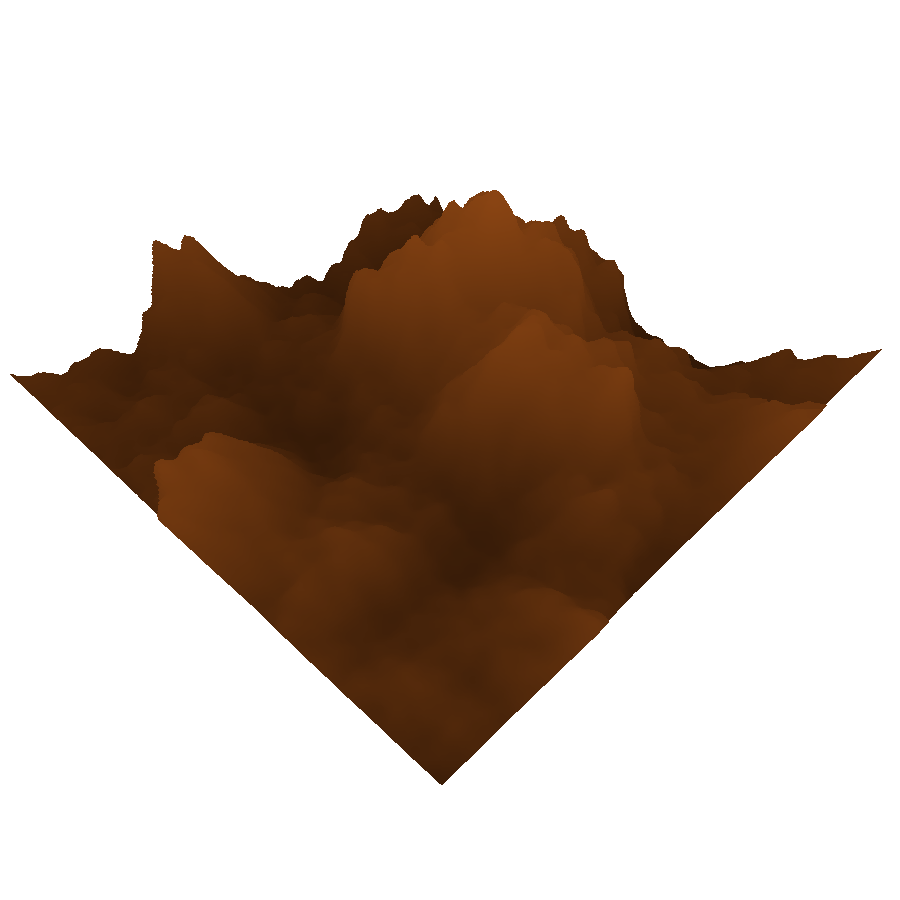
\includegraphics[width=0.6\linewidth, trim=0 110 0 170, clip]{images/terreno.png}
  \caption{Malha 3D de um terreno gerado pela Topograf (ruído
  \texttt{B} da Listagem~\ref{lst:exemplo}).}
  \label{fig:mapa}
\end{figure}

As tabelas usadas são as de células regulares do
Transvoxel~\cite{lengyel_transvoxel}, que correspondem aos casos do
Marching Cubes. O Transvoxel também define células de transição entre
níveis de detalhe diferentes, mas, como o volume é extraído em uma única
resolução, elas não são necessárias.

\subsection{Estrutura de um tradutor}\label{sec:compiladores}
Um tradutor, seja um compilador ou um interpretador, pode ser dividido
em duas fases: a análise
(\textit{front-end}), que lida com a linguagem de origem, e a síntese
(\textit{back-end}), que produz o resultado na linguagem
alvo. A análise é composta por três etapas. Na análise
léxica, o \textit{scanner} agrupa os caracteres do programa em
\textit{tokens}. Na análise sintática, o \textit{parser} verifica se a
sequência de \textit{tokens} segue a gramática livre de contexto da
linguagem e constrói uma árvore sintática abstrata (AST), usada como
representação intermediária. Na análise semântica, a AST e a tabela de
símbolos são usadas para verificar se o programa é consistente com a
definição da linguagem, por exemplo quanto aos tipos de cada
expressão~\cite{ladeira, cooper2014}.

Essas etapas podem ser geradas por ferramentas. O Flex gera o
\textit{scanner} a partir de expressões regulares que descrevem os
\textit{tokens}, e o Bison gera, a partir da gramática, um
\textit{parser} LALR, uma variante da análise ascendente
LR. A partir da mesma AST, um tradutor pode oferecer mais
de um \textit{back-end}: um interpretador, que executa o programa
diretamente, ou um gerador de código, que o traduz para outra
linguagem~\cite{ladeira, grune2012}. A Topograf segue essa organização, com os dois
\textit{back-ends} (Seção~\ref{sec:implementacao}).

%% =====================================================================
%% 3. A LINGUAGEM  (~1,6 pag.)
%% =====================================================================
\section{A Linguagem Topograf}\label{sec:linguagem}

\subsection{Visão geral}\label{sec:visao}
Um programa Topograf é uma sequência de comandos terminados por
ponto e vírgula, em três grupos: o cabeçalho, as declarações de ruído e
os comandos de saída. A Listagem~\ref{lst:exemplo} mostra um programa
completo.

O cabeçalho \texttt{terrain} (linha 1) é obrigatório, aparece uma única
vez e vem antes de qualquer outro comando. Ele define a grade comum a
todos os ruídos do programa, com \texttt{width} $\times$ \texttt{length}
pontos, e a altura máxima \texttt{height}, em \textit{voxels}, usada
apenas na visualização 3D. Como todos os ruídos compartilham a mesma
grade, operações entre ruídos nunca envolvem dimensões diferentes.

As linhas 3 e 4 declaram, com \texttt{perlin}, ruídos primitivos, cada um um gerador Perlin
configurado por parâmetros nomeados, que correspondem aos da
Seção~\ref{sec:perlin}; os omitidos assumem valores padrão, que são
4 para \texttt{frequency}, 2 para \texttt{lacunarity}, $0{,}5$ para
\texttt{persistence}, 3 para \texttt{octaves}, 1 para
\texttt{amplitude} e \texttt{exponent}, 250 para \texttt{wave} e 0
para \texttt{seed}. As linhas 6
e 7 declaram, com \texttt{noise}, ruídos compostos, definidos por expressões sobre ruídos já
declarados: \texttt{grama} é \texttt{A} com a altura reduzida a 70\%, e
\texttt{montanhas} mantém apenas os pontos de \texttt{B} acima de
$0{,}35$, escalados por $0{,}8$.

As linhas 9 a 11 são comandos de saída. O \texttt{display} abre uma
janela 3D com uma camada por expressão, cada uma com sua cor; a
expressão \texttt{(0.35)} é um campo constante e, em ciano, funciona
como um plano de água. A palavra \texttt{depth} escurece as
partes baixas de cada camada. Os comandos \texttt{export} gravam um
ruído como imagem PNG em tons de cinza ou, com \texttt{octaves}, uma
imagem por oitava de um ruído primitivo.

\begin{lstlisting}[caption={Exemplo de uso da Topograf.}, label={lst:exemplo}, float=t]
terrain(width: 256, length: 256, height: 256);

perlin A(frequency: 1, octaves: 6, seed: 28082004);
perlin B(frequency: 2, octaves: 5, seed: 28082004, exponent: 2);

noise grama = A * 0.7;
noise montanhas = above(B, 0.35) * 0.8;

display grama#green, montanhas#white, (0.35)#cyan depth;
export montanhas as "resultados/montanhas.png";
export octaves B to "resultados/camadas/";
\end{lstlisting}

\subsection{Sintaxe}\label{sec:sintaxe}
A Listagem~\ref{lst:gramatica} resume a gramática na notação do Bison.
Um programa é o cabeçalho seguido de zero ou mais comandos, e a
gramática impõe que \texttt{terrain} venha primeiro e apareça uma única
vez. As funções embutidas, como \texttt{max}, \texttt{above} e
\texttt{mix}, não têm produções próprias: todas são reconhecidas
pela regra geral \texttt{IDENT '(' args ')'}, e a análise semântica
confere o nome e a aridade. Assim, acrescentar uma função não altera a
gramática.

As expressões usam uma gramática ambígua, \texttt{expr op expr}, e a
ambiguidade é resolvida por declarações de precedência:
\texttt{+} e \texttt{-} têm a mesma precedência, menor que a de
\texttt{*} e \texttt{/}, e todos associam à esquerda. Com isso, o Bison
gera o \textit{parser} LALR sem conflitos não resolvidos, o que o
próprio arquivo da gramática exige (\texttt{\%expect 0}). A divisão é
aceita pela sintaxe apenas para ser rejeitada na análise semântica, com
uma mensagem mais clara que um erro sintático. Não há sinal negativo:
números são sempre literais não negativos.

Duas decisões ficam no léxico. A primeira é a cor de uma camada do
\texttt{display}, escrita colada à expressão, como \texttt{A\#red}. Como
as expressões regulares do Flex não enxergam o que veio antes do
\textit{token}, o analisador léxico guarda se o último trecho consumido
foi espaço ou comentário e, nesse caso, rejeita a cor com um erro
específico. A segunda é \texttt{octaves}, que é palavra-chave no
comando \texttt{export octaves} e também nome de parâmetro dos
ruídos primitivos; a regra \texttt{nome\_param} aceita tanto um
identificador quanto essa palavra-chave.

Erros léxicos e sintáticos interrompem a análise no primeiro erro, com
linha, coluna e uma mensagem em português que indica o \textit{token}
encontrado e os esperados.

\begin{lstlisting}[language={}, caption={Gramática da Topograf (notação Bison, simplificada).}, label={lst:gramatica}, float=t, numbers=none]
programa : cabecalho comandos ;
cabecalho: TERRAIN '(' params ')' ';' ;
comando  : PERLIN IDENT '(' params ')' ';'
         | NOISE IDENT '=' expr ';'
         | DISPLAY camadas opt_prof ';'
         | EXPORT IDENT AS STRING ';'
         | EXPORT OCTAVES IDENT TO STRING ';' ;
param    : nome_param ':' NUMERO ;
nome_param: IDENT | OCTAVES ;
expr     : expr '+' expr | expr '-' expr
         | expr '*' expr | expr '/' expr
         | '(' expr ')' | NUMERO | IDENT
         | IDENT '(' args ')' ;
camada   : expr opt_cor ;
\end{lstlisting}

\subsection{Tipos e semântica}\label{sec:semantica}
A Topograf distingue três tipos de valor. Um ruído primitivo é um
gerador Perlin declarado com \texttt{perlin} e parâmetros; um ruído
composto é definido com \texttt{noise} e uma expressão; um número é um
literal. Primitivos e compostos são campos, que atribuem um valor em
$[0,1]$ a cada ponto da grade. A distinção entre eles é feita já pela
sintaxe e só importa em \texttt{export octaves}, que exige um
primitivo, pois só ele tem oitavas.

Todas as operações são ponto a ponto: sendo $(i,j)$ o índice de um
ponto da grade de \texttt{width} $\times$ \texttt{length}, o valor em
$(i,j)$ depende apenas
dos valores dos operandos em $(i,j)$. A Tabela~\ref{tab:operadores}
lista os operadores. Todo resultado é limitado a $[0,1]$, de modo que os
campos são fechados sob todas as operações: qualquer expressão aceita
pela análise semântica produz um mapa de altura válido. Um número em
posição de ruído é promovido a campo constante, também limitado a
$[0,1]$, o que permite escrever limiares como \texttt{above(B, 0.35)} ou
deslocamentos como \texttt{A + 0.2}. A exceção é o produto, em que o
literal atua como fator de escala e pode ser maior que 1, como em
\texttt{2 * A}.

A análise semântica percorre a AST com uma tabela de símbolos que
guarda o nome, o tipo e a linha de declaração de cada ruído, e verifica
as seguintes regras:
\begin{itemize}
  \item todo nome é declarado antes do uso, uma única vez, e não
        coincide com o de uma função embutida;
  \item os parâmetros de \texttt{terrain} e dos primitivos existem, não
        se repetem e respeitam seus domínios: as dimensões e
        \texttt{wave} são inteiros positivos, \texttt{octaves} é inteiro
        e maior ou igual a 1, \texttt{seed} é inteiro e os demais são
        positivos; como a gramática não tem sinal negativo, valores
        negativos já são rejeitados na análise sintática;
  \item no produto, ao menos um lado é um literal numérico, o que
        exclui ruído $\times$ ruído, e a divisão é sempre rejeitada;
  \item cada função recebe o número correto de argumentos e, em
        \texttt{mix}, os pesos são literais e não ambos nulos;
  \item \texttt{export octaves} recebe um primitivo, e
        \texttt{display} exige \texttt{height} no cabeçalho.
\end{itemize}
Um literal é um nó numérico da AST. Como parênteses não criam nós,
\texttt{(2)} é literal, mas \texttt{2*3} não é.

Ao contrário dos erros léxicos e sintáticos, os erros semânticos são
acumulados: a análise continua após o primeiro erro, todos são
reportados juntos, com linha e coluna, e o programa não é executado se
houver algum.

\begin{table}[htb]
  \caption{Operadores da Topograf e seu valor em cada ponto $(i,j)$.}
  \label{tab:operadores}
  \centering
  \small
  \begin{tabular}{ll}
    \toprule
    \textbf{Expressão} & \textbf{Resultado} \\
    \midrule
    \texttt{A + B}              & $\min(1, A + B)$ \\
    \texttt{A - B}              & $\max(0, A - B)$ \\
    \texttt{k * A}              & $\operatorname{clamp}_{[0,1]}(k\,A)$ \\
    \texttt{max(A, B)}          & $\max(A, B)$ \\
    \texttt{min(A, B)}          & $\min(A, B)$ \\
    \texttt{above(A, B)}        & $A$ se $A > B$, senão $0$ \\
    \texttt{below(A, B)}        & $A$ se $A < B$, senão $0$ \\
    \texttt{avg(A, B)}          & $(A + B)/2$ \\
    \texttt{mix(A,B,nA,nB)}     & $(A\,n_A + B\,n_B)/(n_A + n_B)$ \\
    \bottomrule
  \end{tabular}
\end{table}

\subsection{Saídas}\label{sec:saidas}
O comando \texttt{export X as "terreno-final.png"} grava o ruído \texttt{X},
primitivo ou composto, como uma imagem em tons de cinza com
\texttt{width} $\times$ \texttt{length} \textit{pixels}, em que o valor
de cada ponto em $[0,1]$ é levado à faixa de 0 a 255. O comando
\texttt{export octaves X to "camadas/"} aceita apenas primitivos e grava
uma imagem por oitava, sem o peso da persistência, o que permite
inspecionar a contribuição de cada escala separadamente. Em ambos os
casos, os diretórios que faltam são criados.

O comando \texttt{display} abre uma janela com a visualização 3D. Cada
expressão da lista é uma camada, convertida em malha como na
Seção~\ref{sec:mc} e desenhada com a cor indicada após \texttt{\#}, por
código hexadecimal ou por uma de dez cores nomeadas; sem cor, a camada
é cinza. As camadas são sobrepostas na mesma cena e, onde coincidem, a
posterior fica por cima. A opção \texttt{depth} escurece as
partes baixas de cada camada, o que realça o relevo. Cada
\texttt{display} abre a sua própria janela, e todas ficam abertas ao
mesmo tempo.

A ordem dos comandos de saída não altera o resultado: todas as
exportações são feitas antes de qualquer janela ser aberta, de modo que
os arquivos já estão gravados enquanto o usuário inspeciona o terreno.

%% =====================================================================
%% 4. IMPLEMENTACAO  (~1,0 pag.)
%% =====================================================================
\section{Implementação}\label{sec:implementacao}

\subsection{Tecnologias utilizadas}\label{sec:tecnologias}
A Topograf foi implementada em C++20. O analisador léxico é gerado pelo
Flex (versão 2.6 ou superior) e o sintático pelo Bison (3.8 ou
superior), com o esqueleto em C++. O projeto é construído com CMake, e
os testes automatizados rodam com o CTest. As imagens são gravadas com
a biblioteca \texttt{stb\_image\_write}, e a visualização usa o motor
gráfico IFCG, construído sobre OpenGL, GLFW e GLM
(Seção~\ref{sec:gerador}).

\subsection{Arquitetura do tradutor}\label{sec:arquitetura}
A Figura~\ref{fig:pipeline} mostra o fluxo. O \textit{scanner} gerado
pelo Flex entrega os \textit{tokens} ao \textit{parser} gerado pelo
Bison, que usa o esqueleto em C++ e constrói a AST com nós alocados em
\texttt{std::unique\_ptr}. A análise semântica percorre a AST, monta a
tabela de símbolos e devolve a lista de erros. Sem erros, o programa
segue para um dos dois \textit{back-ends}: por padrão, é interpretado;
com a opção \texttt{-o}, é traduzido para C++ e compilado pelo
compilador do sistema, ligado à biblioteca de \textit{runtime} da
Topograf. Opções adicionais interrompem o fluxo após a análise sintática
ou a semântica e imprimem a AST ou a tabela de símbolos, o que é usado
nos testes.

\begin{figure}[htb]
  \centering
  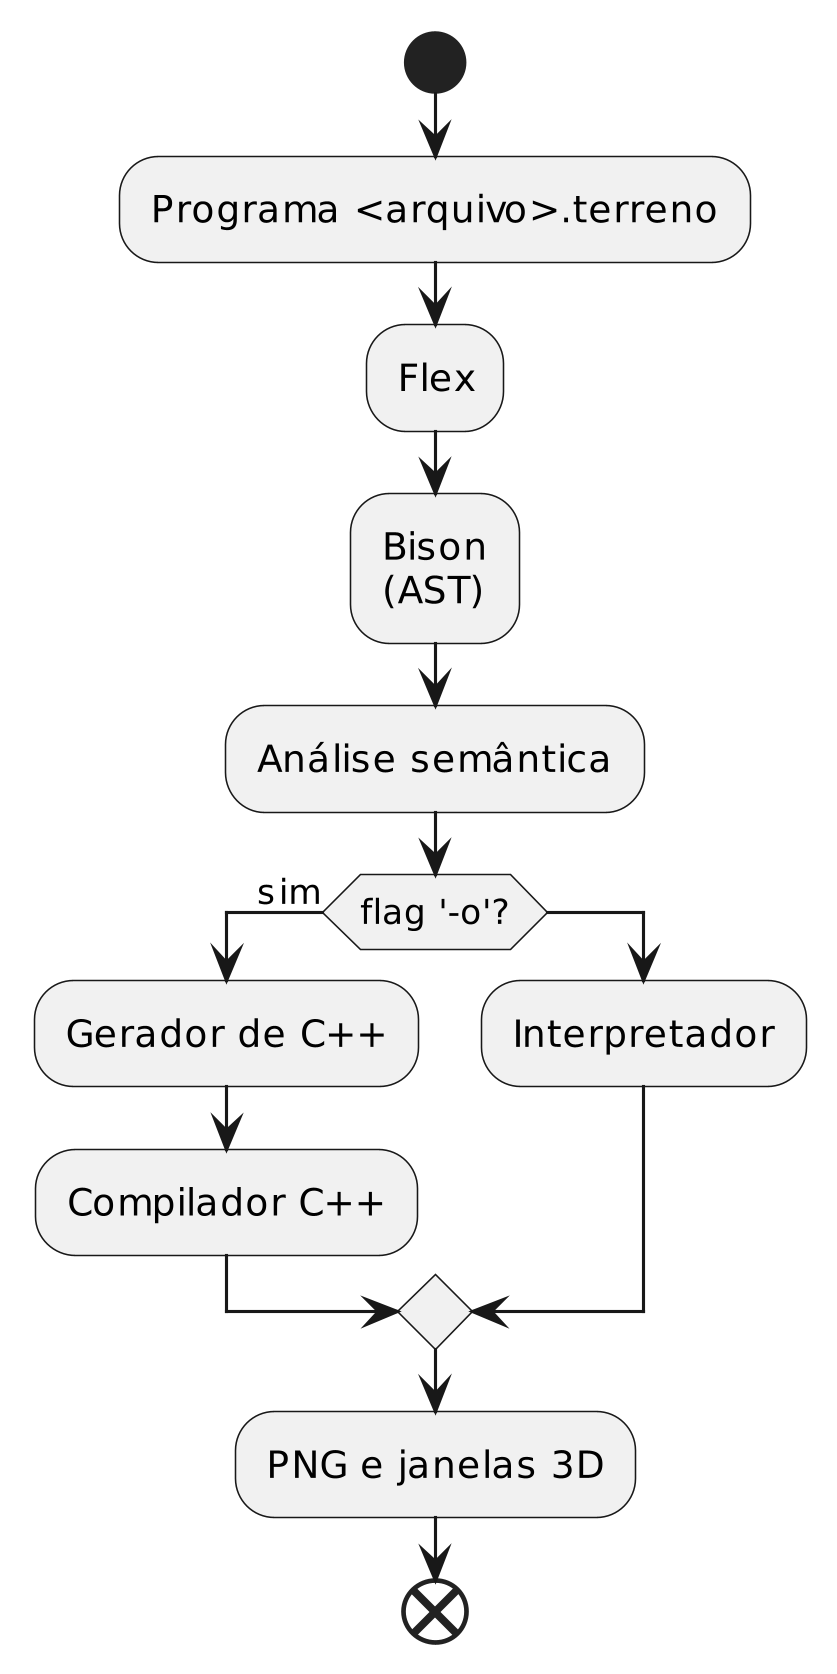
\includegraphics[width=0.5\linewidth]{images/pipeline.png}
  \caption{Fluxo da Topograf. Os dois \textit{back-ends} usam o mesmo \textit{runtime}.}
  \label{fig:pipeline}
\end{figure}

\subsection{Avaliação e geração de código}\label{sec:avaliacao}
O interpretador percorre a AST diretamente, sem gerar código. Ele
executa os comandos de saída e avalia apenas os ruídos que eles usam,
sob demanda: ao encontrar um nome, gera o primitivo ou avalia a
expressão do composto e guarda o campo em \textit{cache}, de modo que
cada ruído é calculado uma única vez, mesmo que apareça em várias
expressões. A avaliação de uma expressão é recursiva, e cada nó produz
um campo inteiro: um literal vira campo constante, e um operador combina
ponto a ponto os campos dos filhos com a função correspondente do
\textit{runtime}. O gerador de
código, em vez disso, traduz cada primitivo em uma chamada ao gerador
de ruído e cada composto em um único laço sobre a grade, com a
expressão inteira embutida, sem campos intermediários. Para
\texttt{montanhas}, na Listagem~\ref{lst:exemplo}, o corpo do laço é
\begin{center}
\scriptsize
\texttt{v\_montanhas[i] = prt::scale(0.8f, prt::above(v\_B[i], prt::c01(0.35f)));}
\end{center}
(com as conversões numéricas simplificadas). Os dois \textit{back-ends}
chamam as mesmas funções do \textit{runtime} para cada operação, e o
código gerado é compilado com \texttt{-ffp-contract=off}, que impede o
compilador de fundir multiplicações e somas em uma única instrução e
alterar o arredondamento. Assim, o executável e o interpretador devem
produzir os mesmos valores, o que é verificado na
Seção~\ref{sec:resultados}.

\subsection{Gerador de terrenos 3D}\label{sec:gerador}
Na visualização, cada coluna recebe
$\operatorname{round}(1 + h\,(H-1))$ \textit{voxels}, em que $h$ é o
valor do ruído e $H$ o \texttt{height}, de modo que toda coluna tem ao
menos um \textit{voxel}. Cada camada do \texttt{display} gera uma malha
própria pelo Marching Cubes da Seção~\ref{sec:mc}; vértices sobre a
mesma aresta são compartilhados entre células vizinhas por meio de uma
tabela \textit{hash}. Com \texttt{depth}, a cor de cada vértice é
multiplicada por $0{,}35 + 0{,}65\,t$, em que $t$ é a altura do vértice
normalizada entre a menor e a maior coluna da camada. Para evitar
\textit{z-fighting}, a camada $i$ é deslocada $0{,}05\,i$ para cima, o
que faz a posterior aparecer por cima onde as camadas coincidem.

As malhas são desenhadas pelo IFCG, um motor gráfico em
OpenGL~\cite{learnopengl}\footnote{\anonfinal{Endereço omitido para avaliação cega.}{\url{https://github.com/andrevbastos/ifcg}}}
que admite uma
única janela por processo e exige a \textit{thread} principal. Por isso,
cada \texttt{display} roda em um processo filho criado com
\texttt{fork}, e o processo pai espera todas as janelas serem fechadas.
Antes de abrir a janela, cada filho gera as malhas em paralelo com o
\textit{thread pool} do IFCG, implementado com \texttt{std::jthread} do
C++20~\cite{williams2019}. O \textit{pool} é criado já no filho, pois o
\texttt{fork} copia apenas a \textit{thread} que o chamou. A grade de
cada camada é dividida em fatias ao longo de $z$, processadas como
tarefas independentes, cada uma com sua própria tabela \textit{hash}; na
junção, os vértices da fronteira entre fatias vizinhas são unificados na
mesma ordem da versão sequencial, de modo que a malha resultante é
idêntica.

%% =====================================================================
%% 5. RESULTADOS  (~0,9 pag.)
%% =====================================================================
\section{Resultados}\label{sec:resultados}
A Figura~\ref{fig:terreno} mostra as saídas do programa da
Listagem~\ref{lst:exemplo}. Na visualização 3D, a camada verde é
\texttt{grama}, o plano ciano é o campo constante $0{,}35$ e a camada
branca é \texttt{montanhas}. Como \texttt{above} zera os pontos de
\texttt{B} abaixo do limiar, \texttt{montanhas} passa de 0 a mais de
$0{,}28$ entre pontos vizinhos, e essa descontinuidade aparece como
paredes verticais que sobem da base, em cinza escuro por causa da
\texttt{depth}. A figura também mostra o mapa de altura de
\texttt{B}, gravado por \texttt{export}, e suas cinco oitavas, em que
a frequência dobra a cada camada.

\begin{figure}[htb]
  \centering
  \begin{tabular}{@{}c@{\hspace{2mm}}c@{}}
    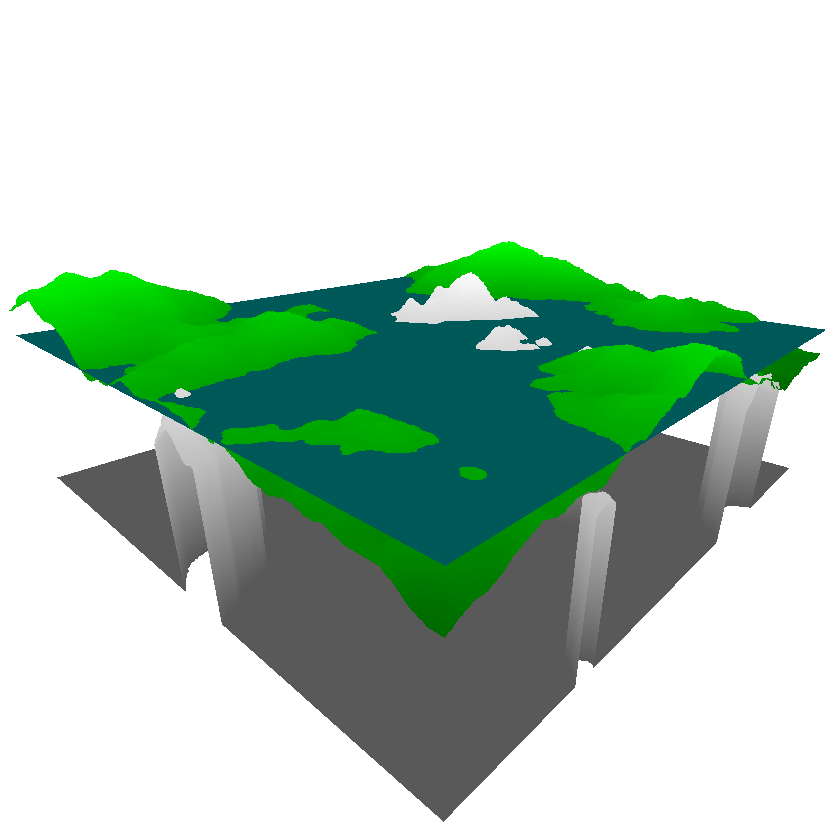
\includegraphics[width=0.52\linewidth, trim=0 60 0 220, clip]{images/display.png} &
    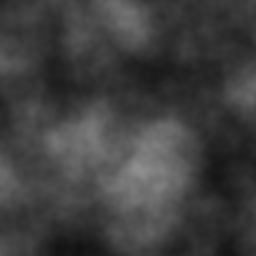
\includegraphics[width=0.40\linewidth]{images/export.png} \\
    \small (a) & \small (b)
  \end{tabular}\\[1mm]
  \begin{tabular}{@{}c@{\hspace{1mm}}c@{\hspace{1mm}}c@{\hspace{1mm}}c@{\hspace{1mm}}c@{}}
    
\includegraphics[width=0.185\linewidth]{images/camadas/export_octave_0.png} &
    
\includegraphics[width=0.185\linewidth]{images/camadas/export_octave_1.png} &
    
\includegraphics[width=0.185\linewidth]{images/camadas/export_octave_2.png} &
    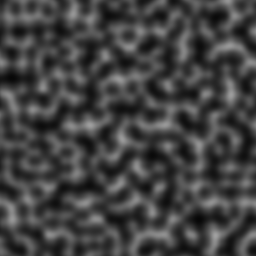
\includegraphics[width=0.185\linewidth]{images/camadas/export_octave_3.png} &
    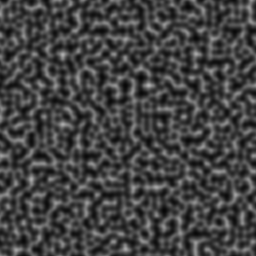
\includegraphics[width=0.185\linewidth]{images/camadas/export_octave_4.png} \\
    \multicolumn{5}{c}{\small (c)}
  \end{tabular}
  \caption{Saídas do programa da Listagem~\ref{lst:exemplo}: (a) janela do
  \texttt{display}; (b) mapa de altura de \texttt{B}; (c) oitavas 0 a 4
  de \texttt{B}.}
  \label{fig:terreno}
\end{figure}

A implementação é verificada por uma suíte de 40 testes automatizados,
todos aprovados: 22 de sintaxe e 11 de semântica, com programas
válidos e inválidos cuja saída é comparada à esperada; um teste de
avaliação, com 34 verificações; dois de exportação; e quatro de
compilação. A Tabela~\ref{tab:validacao} mostra parte das verificações
de avaliação: com $A$ e $B$ fixados em dois pontos, cada operador
produz o valor da Tabela~\ref{tab:operadores}, com tolerância de
$10^{-6}$. A tolerância é necessária porque valores como $0{,}2$ não
têm representação exata em ponto flutuante, e cada operação acrescenta
um pequeno erro de arredondamento. Três dos testes de compilação geram o executável, executam
o executável e o interpretador e exigem o mesmo código de saída e
arquivos idênticos byte a byte, o que confirma que os dois
\textit{back-ends} são equivalentes nesses programas.

\begin{table}[htb]
  \caption{Valores obtidos com $A = [0{,}2;\ 0{,}8]$ e $B = [0{,}5;\ 0{,}5]$.}
  \label{tab:validacao}
  \centering
  \small
  \begin{tabular}{@{}ll@{\hspace{6mm}}ll@{}}
    \toprule
    \textbf{Expressão} & \textbf{Valor} & \textbf{Expressão} & \textbf{Valor} \\
    \midrule
    \texttt{A + B}       & $[0{,}7;\ 1{,}0]$ & \texttt{above(A, B)}  & $[0{,}0;\ 0{,}8]$ \\
    \texttt{A - B}       & $[0{,}0;\ 0{,}3]$ & \texttt{below(A, B)}  & $[0{,}2;\ 0{,}0]$ \\
    \texttt{max(A, B)}   & $[0{,}5;\ 0{,}8]$ & \texttt{avg(A, B)}    & $[0{,}35;\ 0{,}65]$ \\
    \texttt{min(A, B)}   & $[0{,}2;\ 0{,}5]$ & \texttt{mix(A, B, 30, 70)} & $[0{,}41;\ 0{,}59]$ \\
    \bottomrule
  \end{tabular}
\end{table}

%% =====================================================================
%% 6. DISCUSSAO  (~0,3 pag.)
%% =====================================================================
\section{Discussão}\label{sec:discussao}
A restrição de que todo campo fique em $[0,1]$ simplifica a linguagem:
nenhuma expressão aceita produz um mapa de altura inválido, e o usuário
não precisa normalizar resultados intermediários. O preço é que
operações cujo resultado sai do intervalo, como somas de vários ruídos,
saturam em 1 em vez de serem reescaladas. Outras escolhas limitam a
expressividade: ruído $\times$ ruído, divisão e pesos variáveis ficaram
fora do escopo, de modo que não é possível, por exemplo, usar um ruído
como máscara multiplicativa de outro.

Os resultados também mostram efeitos que o usuário precisa conhecer.
Os operadores de limiar, como \texttt{above}, criam descontinuidades que
a visualização exibe como paredes verticais
(Figura~\ref{fig:terreno}a). Além disso, o ruído Perlin não ocupa todo
o intervalo: com uma oitava e amplitude e expoente iguais a 1, como
$|P| \le \sqrt{2}/2$, os valores ficam em aproximadamente
$[0{,}15;\ 0{,}85]$, o que afeta a escolha de limiares.

Há ainda limitações de implementação e de avaliação. O terreno é um
mapa de altura e, portanto, não representa cavidades nem saliências. A
abertura de uma janela por processo depende de \texttt{fork} e,
portanto, de sistemas POSIX. O desempenho do interpretador, do código
gerado e da geração de malhas não foi medido, e a Topograf não foi
comparada com bibliotecas de ruído ou editores existentes, nem avaliada
com usuários.

\section{Conclusões e Trabalhos Futuros}\label{sec:conclusao}
Este artigo apresentou a Topograf, uma DSL para compor ruídos Perlin e
gerar terrenos. A linguagem fecha todas as operações em $[0,1]$, rejeita
na análise semântica as composições sem significado no domínio e
oferece dois \textit{back-ends}, um interpretador e um tradutor para
C++, cujos resultados foram verificados como idênticos byte a byte nos
testes. As camadas de um programa podem ser exportadas como imagens ou
visualizadas em 3D por meio de Marching Cubes.

Como trabalhos futuros, no gerador de terrenos, pretende-se representar
cavidades e saliências com ruído 3D e volumes gerados diretamente, sem
passar por um mapa de altura; incluir erosão; oferecer transições
suaves no lugar dos limiares abruptos, que hoje produzem paredes
verticais; usar as células de transição do Transvoxel para níveis de
detalhe; e exportar as malhas. Na linguagem, pretende-se admitir
operações entre ruídos e pesos variáveis, que permitiriam usar um ruído
como máscara de outro, outros geradores de ruído, constantes nomeadas e
funções definidas pelo usuário, além de atualizar a visualização a cada
alteração do programa. Também se pretende medir o desempenho dos dois
\textit{back-ends} e comparar a linguagem com ferramentas existentes.

\section*{Agradecimentos}
\anonfinal{Agradecimentos omitidos para fins de avaliação cega.}{Os autores agradecem ao Instituto Federal Catarinense (IFC), Campus Blumenau, pelo apoio ao desenvolvimento deste trabalho.}

\section*{Declaração de Uso de Inteligência Artificial}
Os autores declaram que o assistente de inteligência artificial Claude Code foi
utilizado para a revisão textual e ortográfica, a estruturação conceitual das
ideias e a formatação das tabelas deste artigo. Ressalta-se que toda a
concepção do estudo, implementação do software, execução dos experimentos e
análise científica são de inteira responsabilidade dos autores.

\bibliographystyle{ACM-Reference-Format}
\bibliography{topograf}

\end{document}
